\input{../../header.tex}

\usepackage{tikz}
\usetikzlibrary{chains}
\usetikzlibrary{shapes.geometric}

\usepackage{booktabs}

\hypersetup{
    pdftitle=
}

\subject{Praktikumsprotokoll}
\title{Nukleare Elektronik und Lebensdauermessung}
\subtitle{Versuch P525 -- Universität Bonn}
\author{
    Martin Ueding \\ \small{\href{mailto:mu@martin-ueding.de}{mu@martin-ueding.de}}
    \and
    Lino Lemmer
}
\publishers{Tutor: Philipp Hoffmeister}

\begin{document}

\maketitle

\tableofcontents

\chapter{Theorie}

\section{Zerfallsschema von ${}^{22}\text{Na}$ und ${}^{133}\text{Ba}$}

Das Moseley'sche Gesetz gibt die Frequenz der charakteristischen Röntgenstrahlung eines Kerns mit Kernladung $Z$ an: \parencite[(17.10)]{meschede-gerthsen_24}
\begin{equation}
    \label{eq:moseley}
    E = h \nu = \frac 34 R_\infty c \cdot (Z - 1)^2.
\end{equation}

Nach dem Moseley'schen Gesetz \eqref{eq:moseley} ist die Energie der $K_\alpha$-Röntgenstrahlung
von Barium \SI{<< E_K_alpha_Ba_keV >>}{\kilo\electronvolt}.

\section{Instrumente}

\subsection{Szintillationsspektrometer}

\subsection{Photomultiplier (MP)}

\subsection{Splitter}

\subsection{Verstärker}

Der Verstärker/Operationsverstärker (engl. Amplifier) ist ein elektrisches
Bauteil, welches die Aufgabe hat ein eingehendes Signal zu verstärken. Es gibt
Strom-, Spannungs- und Ladungsempfindliche Verstärker, je nach der Art des
verstärkten Signales.

%TODO: Funktionsweise

\subsection{Constant Fraction Diskriminator (CFD)}

\subsection{Einkanalanalysator (SCA)}

\subsection{Vielkanalanalysator (MCA)}

\subsection{Koinzidenzeinheit}

\subsection{Zeit-Impulshöhe-Konverte (TAC)}

\chapter{Durchführung}


Für unsere Blockschaltbilder benutzen wir folgende Notation:

\begin{tabular}{lc}
    Element & Symbol \\
    \midrule
    Analoges Signal & 
        \begin{tikzpicture} \draw[->] (0, 0) -- ++(1, 0); \end{tikzpicture}
    \\
    Digitales Signal & 
        \begin{tikzpicture} \draw[->, dashdotted] (0, 0) -- ++(1, 0); \end{tikzpicture}
    \\
    Gerät & 
        \begin{tikzpicture} \node[draw, rectangle, minimum size=1ex, draw] {}; \end{tikzpicture}
    \\
    Verstärker &
        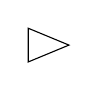
\begin{tikzpicture} \node[draw, isosceles triangle, minimum size=1ex, draw] {}; \end{tikzpicture}
\end{tabular}

\parencite{Bieling/K125}

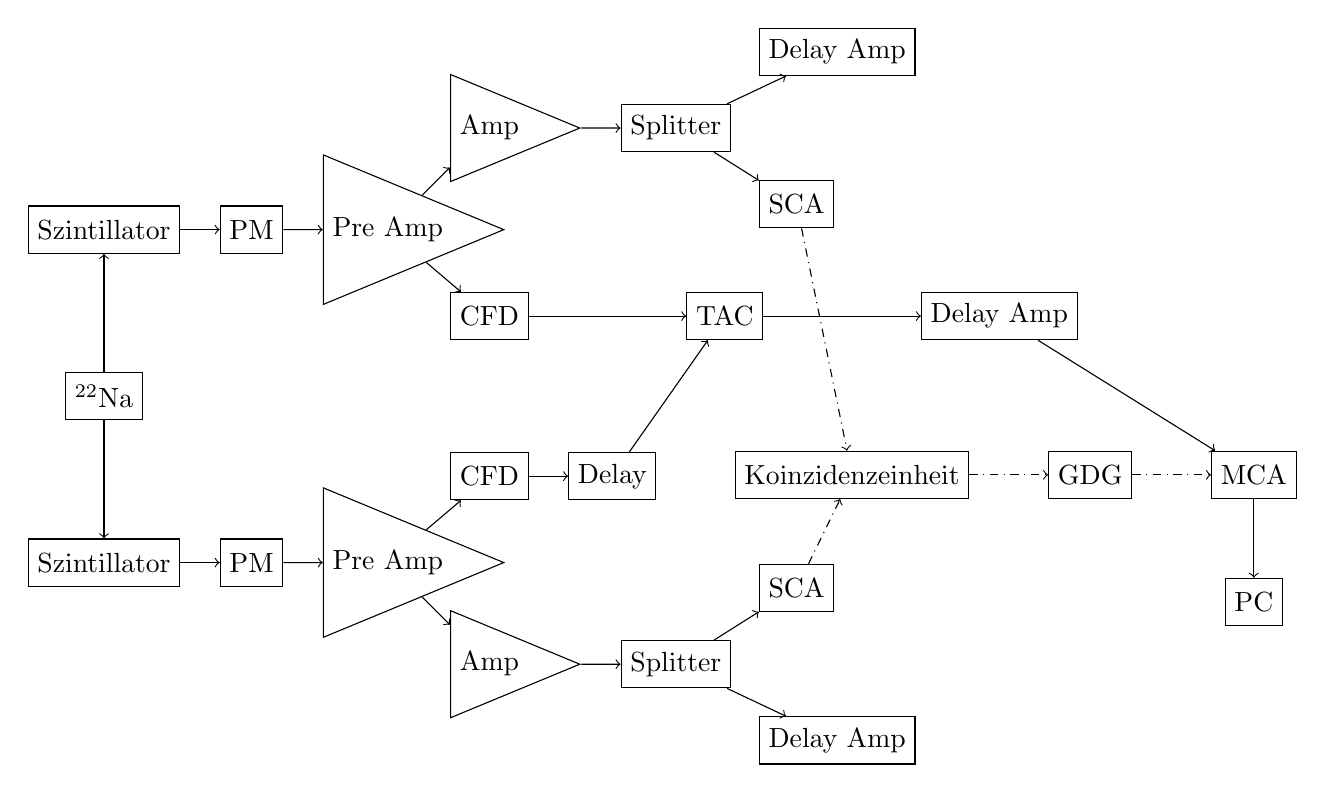
\begin{tikzpicture}[
        device/.style={
            rectangle,
            minimum size=6mm,
            draw=black
        },
        amp/.style={
            isosceles triangle,
            minimum size=6mm,
            draw=black
        },
    ]

    \node[device] (koinzidenz) at (9.5, -1) {Koinzidenzeinheit};
    \node[device] (gdg) [right=of koinzidenz] {GDG};
    \node[device] (mca) [right=of gdg] {MCA};
    \node[device] (pc) [below=of mca] {PC};

    \begin{scope}[start chain, node distance=5mm, every node/.style={join}, every join/.style={->}]
        \node[device, on chain] (22Na) at (0, 0) {$^{22}\mathrm{Na}$};

        \begin{scope}[start branch=22Na]
            \node[device, on chain=going below, node distance=1.5cm] (Szintillator1) {Szintillator};
            \node[device, on chain] (PM2) {PM};
            \node[amp, on chain] (PA2) {Pre Amp};

            \begin{scope}[start branch=PA2]
                \node[amp, on chain=going below right] (amp2) {Amp};
                \node[device, on chain] (splitter2) {Splitter};
                \begin{scope}[start branch=splitter2]
                    \node[device, on chain=going below right] (delay2) {Delay Amp};
                \end{scope}
                \begin{scope}[start branch=splitter2]
                    \node[device, on chain=going above right] (sca2) {SCA};
                \end{scope}

            \end{scope}
            \node[device, on chain=going above right] (cfd2) {CFD};
            \node[device, on chain] (cfddelay) {Delay};
        \end{scope}

        \node[device, on chain=going above, node distance=1.5cm] (Szintillator1) {Szintillator};
        \node[device, on chain] (PM1) {PM};
        \node[amp, on chain] (PA1) {Pre Amp};

        \begin{scope}[start branch=PA1]
            \node[amp, on chain=going above right] (amp1) {Amp};
            \node[device, on chain] (splitter1) {Splitter};
            \begin{scope}[start branch=splitter1]
                \node[device, on chain=going above right] (delay1) {Delay Amp};
            \end{scope}
            \begin{scope}[start branch=splitter1]
                \node[device, on chain=going below right] (sca1) {SCA};
            \end{scope}
        \end{scope}

        \node[device, on chain=going below right] (cfd1) {CFD};
        \node[device, on chain=going right, node distance=2cm, join=with cfddelay] (tac) {TAC};
        \node[device, on chain=going right, node distance=2cm] (delay3) {Delay Amp};

    \end{scope}

    \begin{scope}[->]
        \draw (delay3) -- (mca);
        \draw (mca) -- (pc);

        \begin{scope}[dashdotted]
            \draw (gdg) -- (mca);
            \draw (sca1) -- (koinzidenz);
            \draw (koinzidenz) -- (gdg);
            \draw (sca2) -- (koinzidenz);
        \end{scope}
    \end{scope}
\end{tikzpicture}

\parencite{Leo/Techniques_Nuclear_Experiments}

\chapter{Auswertung}

\chapter{Ergebnis}

\IfFileExists{\bibliographyfile}{
    \printbibliography
}{}

\end{document}

% vim: spell spelllang=de
